\documentclass[11pt]{article}
\usepackage{courier}
\usepackage{fullpage}
\parindent=0in


%------------------------------------------------------------------
% PROBLEM, PART, AND POINT COUNTING...

% Create the problem number counter.  Initialize to zero.
\newcounter{problemnum}

% Specify that problems should be labeled with arabic numerals.
\renewcommand{\theproblemnum}{\arabic{problemnum}}


% Create the part-within-a-problem counter, "within" the problem counter.
% This counter resets to zero automatically every time the PROBLEMNUM counter
% is incremented.
\newcounter{partnum}[problemnum]

% Specify that parts should be labeled with lowercase letters.
\renewcommand{\thepartnum}{\arabic{problemnum}.\arabic{partnum}}

% Make a counter to keep track of total points assigned to problems...
\newcounter{totalpoints}

% Make counters to keep track of points for parts...
\newcounter{curprobpts}		% Points assigned for the problem as a whole.
\newcounter{totalparts}		% Total points assigned to the various parts.

% Make a counter to keep track of the number of points on each page...
\newcounter{pagepoints}
% This counter is reset each time a page is printed.

% This "program" keeps track of how many points appear on each page, so that
% the total can be printed on the page itself.  Points are added to the total
% for a page when the PART (not the problem) they are assigned to is specified.
% When a problem without parts appears, the PAGEPOINTS are incremented directly
% from the problem as a whole (CURPROBPTS).


%---------------------------------------------------------------------------


% The \problem environment first checks the information about the previous
% problem.  If no parts appeared (or if they were all assigned zero points,
% then it increments TOTALPOINTS directly from CURPROBPTS, the points assigned
% to the last problem as a whole.  If the last problem did contain parts, it
% checks to make sure that their point values total up to the correct sum.
% It then puts the problem number on the page, along with the points assigned
% to it.

\newenvironment{problem}[1]{
% STATEMENTS TO BE EXECUTED WHEN A NEW PROBLEM IS BEGUN:
%
% Increment the problem number counter, and set the current \ref value to that
% number.
\refstepcounter{problemnum}
%
% Add some vspace to separate from the last problem.
\vspace{0.15in} \par
%
\setcounter{curprobpts}{#1} \setcounter{totalparts}{0}	% Reset counters.
%
% Now put in the "announcement" on the page.
{\Large \bf \theproblemnum. \normalsize ({\it \arabic{curprobpts} point\null\ifnum \value{curprobpts} = 1\else s\fi}\/)}
}{
% STATEMENTS TO BE EXECUTED WHEN AN OLD PROBLEM IS ENDED:
%
% If no parts to problem, then increment TOTALPOINTS and PAGEPOINTS for the
% entire problem at once.
\ifnum \value{totalparts} = 0
	\addtocounter{totalpoints}{\value{curprobpts}}	% Add pts to total.
	\addtocounter{pagepoints}{\value{curprobpts}}	% Add pts to page total.
%
% If there were parts for the problem, then check to make sure they total up
% to the same number of points that the problem is worth. Issue a warning
% if not.
\else \ifnum \value{totalparts} = \value{curprobpts}
	\else \typeout{}
	\typeout{!!!!!!!   POINT ACCOUNTING ERROR   !!!!!!!!}
	\typeout{PROBLEM [\theproblemnum] WAS ALLOCATED \arabic{curprobpts} POINTS,}
	\typeout{BUT CONTAINS PARTS TOTALLING \arabic{totalparts} POINTS!}
	\typeout{}
	\fi
\fi
}


%---------------------------------------------------------------------------


% The \newpart command increments the part counter and displays an appropriate
% lowercase letter to mark the part.  It adds points to the point counter
% immediately.  If 0 points are specified, no point announcement is made.
% Otherwise, the announcement is in scriptsize italics.

\newcommand{\newpart}[1]
{
\refstepcounter{partnum}	% Set the current \ref value to the part number.
\hspace{0.05in}		% Indent the part by a quarter inch.
%
% If points are to be printed for this problem (signaled by point value > 0),
% then put them in in scriptsize italics.
\ifnum #1 > 0
	\makebox[0.5in][l]{{\bf \thepartnum.} {\bf ({\it #1 pt\ifnum #1 = 1\else s\fi\/}) \,\,}}
\else
	\makebox[0.25in][l]{({\bf \thepartnum})}
\fi
%
\hspace{0.1in}		% Lead the material away from the part "number".
%
\addtocounter{totalparts}{#1}	% Add points to totalparts for this problem.
\addtocounter{pagepoints}{#1}	% Add points to total for this page.
\addtocounter{totalpoints}{#1}	% Add points to total for entire test.
}


%---------------------------------------------------------------------------



% Just in case you want to skip some numbers in your test...

\newcommand{\skipproblem}[1]{\addtocounter{problemnum}{#1}}



%---------------------------------------------------------------------------


% The \showpoints command simply gives a count of the total points read in up to
% the location at which the command is placed.  Typically, one places one
% \showpoints command at the end of the latex file, just prior to the
% \end{document} command.  It can appear elsewhere, however.

\newcommand{\showpoints}
{
\typeout{}
\typeout{====> A TOTAL OF \arabic{totalpoints} POINTS WERE READ.}
\typeout{}
}


%---------------------------------------------------------------------------



\usepackage{graphicx}
\usepackage[english]{babel}
\usepackage[latin1]{inputenc}
\usepackage{times}
\usepackage[T1]{fontenc}
\usepackage{amsmath}
\usepackage{amssymb}

\newcommand{\argmax}{\mathop{\arg\max}}
\newcommand{\deriv}[1]{\frac{\partial}{\partial {#1}} }
\newcommand{\dsep}{\mbox{dsep}}
\newcommand{\Pa}{\mathop{Pa}}
\newcommand{\ND}{\mbox{ND}}
\newcommand{\De}{\mbox{De}}
\newcommand{\Ch}{\mbox{Ch}}
\newcommand{\graphG}{{\mathcal{G}}}
\newcommand{\graphH}{{\mathcal{H}}}
\newcommand{\setA}{\mathcal{A}}
\newcommand{\setB}{\mathcal{B}}
\newcommand{\setS}{\mathcal{S}}
\newcommand{\setV}{\mathcal{V}}
\DeclareMathOperator*{\union}{\bigcup}
\DeclareMathOperator*{\intersection}{\bigcap}
\DeclareMathOperator*{\Val}{Val}
\newcommand{\mbf}[1]{{\mathbf{#1}}}
\newcommand{\eq}{\!=\!}


\begin{document}

{\centering
  \rule{6.3in}{2pt}
  \vspace{1em}
  {\Large
    CS688: Graphical Models - Spring 2018\\
    Assignment 1\\
  }
  \vspace{1em}
  Assigned: Thursday, Feb 1. Due: Thursday, Feb 15 at 11:59 \\
  \vspace{0.1em}
  \rule{6.3in}{1.5pt}
}
\vspace{1pc}

\textbf{Getting Started:} You should complete the assignment using your own installation of Python 2.7. The only module you are permitted to use in your implementations is Numpy. To get started with the code portions of the assignment, download the assignment archive from Moodle and unzip the file. The data files for this assignment are in the \texttt{data} directory. Code templates are in the \texttt{code} directory. The README file contains additional descriptions of the download.  \textbf{Note}: The autograder uses numpy 1.14. Please use this version of numpy. Note that the autograder environment will fail if you attempt to load other packages.\\

\textbf{Deliverables:} This assignment has two types of deliverables: a report and code files.

\begin{itemize}
\item \textbf{Report: } The solution report will give your answers to the homework questions. Items that you should include in your report are marked with \textbf{(report)}. The maximum length of the report is 5 pages in 11 point font, including all figures and tables. You can use any software to create your report, but your report must be submitted in PDF format. You will upload the PDF of your report to Gradescope under \verb|HW01-Report| for grading. It is strongly recommended that you typeset your report. To assist with this if you wish to use Latex, the Latex source of the handout is also included in the homework archive.

\item \textbf{Code: } The second deliverable is your code. Items that you should include in your code are marked with \textbf{(code)}.  Your code must be Python 2.7 (no iPython notebooks, other formats, or code from other versions of Python). You will upload a zip file (not rar, bz2 or other compressed format) containing all of your code to Gradescope under \verb|HW01-Programming| for autograding.  When unzipped, your zip file should produce a directory called \verb|code|. If your zip file has the wrong structure, the autograder may fail to run.
\end{itemize}
\vspace{0.5em}

\textbf{Academic Honesty Statement:} Copying solutions from external
sources (books, web pages, etc.) or other students is considered
cheating. Sharing your solutions with other students is also
considered cheating. Collaboration indistinguishable from copying is a violation 
of the course's collaboration policy and will be treated as cheating.
Any detected cheating will result in a grade of 0
on the assignment for all students involved, and potentially a grade
of F in the course.\\

\textbf{Introduction:} In this assignment, you will experiment with different aspects of modeling, learning, and applying a Bayesian network to answer probability queries. This assignment focuses on the heart disease diagnosis domain and uses part of a real clinical data set. 
\\

\textbf{Data Set:} The data set consists of 9 variables as described below. The number of each variable corresponds to it's column number in the data set files. There are five sets of training and test data files in standard comma-separated-value (CSV) format. The files are named \textit{data-train-i.txt} and \textit{data-test-i.txt} for $i$ from $1$ to $5$.\\

\begin{center}
\begin{tabular}{|c|c|c|l|}\hline
Number & Name & Description & Values\\ \hline\hline
1 & A   &  Age          & 1:$<45$, 2: $45-55$, 3:$\geq 55$\\ \hline
2 & G   &  Gender                  & 1:Female, 2:Male;\\ \hline
3 & CP  &  Chest Pain & 1:Typical, 2:Atypical, 3:Non-Anginal, 4:None\\ \hline
4 & BP  &  Blood Pressure          & 1:Low, 2:High\\ \hline
5 & CH  &  Cholesterol             & 1:Low, 2:High\\ \hline
6 & ECG &  Electrocardiograph      & 1:Normal, 2:Abnormal\\ \hline
7 & HR  &  Exercise Heart Rate     & 1:Low, 2:High\\ \hline
8 & EIA &  Exercise Induced Angina & 1:No, 2:Yes\\ \hline
9 & HD  & Heart Disease            & 1:No, 2:Yes\\ \hline
\end{tabular}
\end{center}
\vspace{1em}

\textbf{Model: } We will consider applying a Bayesian network
with the following structure to the data set.\\

\begin{center}
    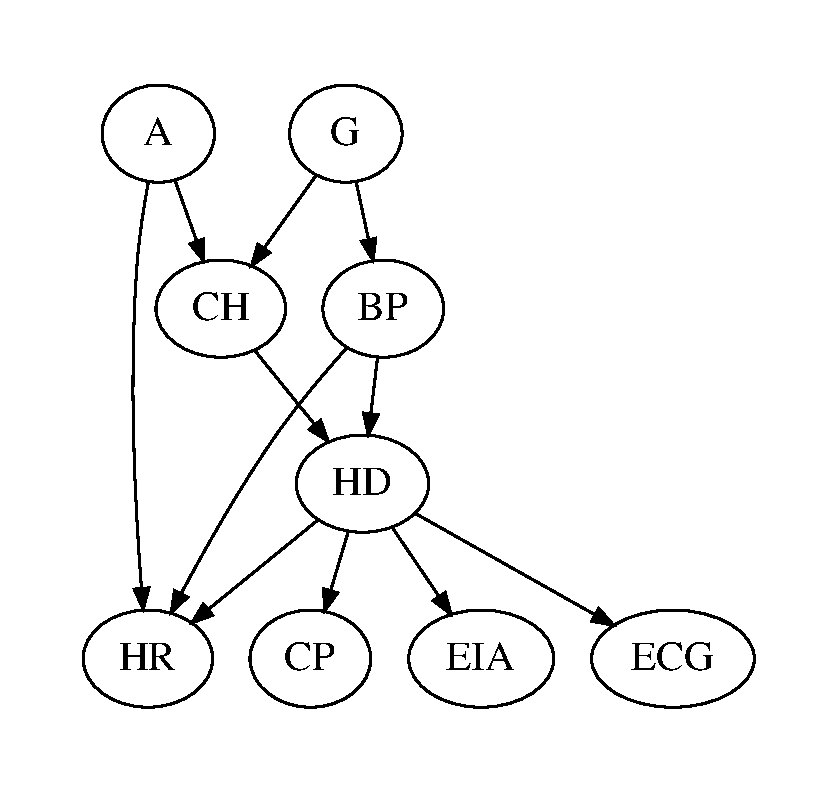
\includegraphics[scale=0.5,trim=10mm 10mm 10mm 10mm,clip]{bn.pdf}
\end{center}

\begin{problem}{10} \textbf{Factorization }:  Write down the factorization of the Bayesian network joint distribution implied by the structure shown above. \textbf{(report)}
\end{problem}

\begin{problem}{10} \textbf{Likelihood Function:} Using the notation for the parameters of CPTs introduced in Lecture 4 (ie: $P_{\theta}(HD=hd|CH=ch,BP=bp)=\theta^{HD}_{hd|ch,bp}$), write down the log likelihood of the Bayesian network model as a function of the parameters $\theta$ given $N$ data cases. \textbf{(report)}
\end{problem}

\begin{problem}{10} \textbf{Maximum Likelihood Estimates: } Using the notation for the parameters of CPTs introduced in Lecture 4, derive the maximum likelihood estimate for the parameter $\theta^{HR}_{L|1,H,Y}$ starting from the log likelihood function. Show all of your work. \textbf{(report)}
\end{problem}

\begin{problem}{15} \textbf{CPT Data Structures} In this question, you will describe and implement conditional probability table data structures for the Bayesian network shown above.\\
	
\newpart{5} To implement the network shown above, you will need to choose a data structure to represent  conditional probability tables. There are many possible choices including classes of your own design. As your answer to this question, explain what data structure you chose to represent CPTs and how it represents CPTs with different numbers of parents and different variable cardinalities. If you implement a custom class, describe its member variables and methods. If you use an existing data structure (lists, array, dictionary, etc.), describe how. (\textbf{report}) \\

\newpart{5}  In the \verb|BayesNet| class contained in \verb|code/bn.py|, implement the \verb|__init__| method. This method should create the set of CPTs needed to represent the above model as member variables according to your approach described in 4.1. You should initialize each CPT to the uniform distribution over the target variable for each setting of the parent variables. (\textbf{code}) \\

\newpart{5} In the \verb|BayesNet| class contained in \verb|code/bn.py|, implement the methods \verb|get| and \verb|set|. These methods provide basic functions to get the current value of a specific probability from a CPT member variable and to set a specific probability in a CPT member variable in a way that is independent of your CPT implementation. (\textbf{code}) 


\end{problem}


\begin{problem}{15} \textbf{Learning:} In this question, you will describe and implement learning for the Bayesian network shown above.\\
	
\newpart{5} To implement maximum likelihood learning for a Bayesian network model, the parameters of each CPT must be estimated from data. This can be accomplished by writing unique code for every CPT in the model. This is conceptually simple, but highly redundant and error prone. It is also possible to write a single general function that can estimate the parameters for any CPT. This is conceptually more complex, but provides much more compact code. As your answer to this question, describe your approach to implementing learning. (\textbf{report})\\

\newpart{10} In the \verb|BayesNet| class contained in \verb|code/bn.py|, implement the \verb|fit| function according to the approach you described in part 1. The \verb|fit| function must implement maximum likelihood parameter estimation for all CPTs in the model. (\textbf{code})

\end{problem}

\begin{problem}{10} \textbf{Probability Queries:} In this question, you will derive and implement solutions to two different
probability queries.\\
	
\newpart{5} For each of the two queries listed below, show how the query can be expressed in terms of the factorized joint distribution for the Bayesian network. Simplify the expressions wherever possible using the conditional independence properties of the network structure. Show your work. (\textbf{report})\\

\textbf{(a)} {\footnotesize $P(CH|A=2,G=M,CP=None,BP=L,ECG=Normal,HR=L,EIA=No,HD=No)$}\\
\textbf{(b)} {\footnotesize $P(BP|A=2,CP=Typical,CH=H,ECG=Normal,HR=H,EIA=Yes,HD=No)$}\\

\newpart{5} In \verb|code/queries.py|, implement the methods \verb|query_5_a| and \verb|query_5_b|. These two functions take an instance of the BayesNet class as input and should compute the query distributions for queries (a) and (b). (\textbf{code})

\end{problem}


\begin{problem}{15} \textbf{Classification:} In this question, we will assess the ability of the model to correctly predict the occurrence of heart disease given the values of all of the other variables in the network. \\

\newpart{5} Write down the probability distribution over the heart disease variable (HD) given the remaining variables for the Bayesian Network model shown above. Simplify the result using the conditional independence properties of the network \textbf{(report)}. \\

\newpart{5} Implement the \verb|predict_hd| method of the BayesNet class in \verb|code/bn.py|. This method will predict if a patient has heart disease or not using the probability of heart disease given the remaining variables as derived in 7.1. Your method should predict Yes (2) if the probability of heart disease if greater than 0.5 and should predict No (1) otherwise \textbf{(code)}.\\

\newpart{5}  We will follow a standard five-fold cross-validation protocol to assess the performance of classifier derived from the model in 7.2. For each training file $i$, use your Bayesian network implementation to learn the parameters of the model, then make predictions for the heart disease variable for each data case $n$ in test file $i$ using the \verb|predict_hd| method. For each test file $i$, compute the prediction accuracy $A_i$ as the number of cases correctly predicted divided by the total number of cases. Lastly, compute the mean prediction accuracy over the five test files (the average of $A_1$ to $A_5$) and the standard deviation of the prediction accuracy over the five test files (the standard deviation of $A_1$ to $A_5$). Report the mean and the standard deviation of the prediction accuracy that you find \textbf{(report)}. Add your code to \textbf{accuracy.py} \textbf{(code)}.
\end{problem}


\begin{problem}{15} \textbf{Modeling:} In this question, you will design, implement and evaluate your own network structure for the heart disease domain. \\

\newpart{2}  Provide a figure showing the graphical model for your network \textbf{(report)}. \\

\newpart{3}  Write down the factorization for your network \textbf{(report)}.\\

\newpart{3}  Briefly describe some of the choices that went into the design of your network \textbf{(report)}.\\

\newpart{5}  Implement your network in \verb|code/bn_custom.py|. The API for this class is identical to that of \verb|code/bn.py|. You must support the \verb|fit|, \verb|get|, \verb|set|, and \verb|predict_hd| methods \textbf{(code)}. \\

\newpart{2}  As in the previous question, apply the five-fold cross-validation protocol to assess and report the mean prediction accuracy of your model, along with its standard deviation. \textbf{(report)}

\end{problem}

\showpoints
\end{document}
